\section{Introduction}
Message oriented middleware (MOM) is highly used in distributed systems.


\section{ActiveMQ}

\section{RabbitMQ}
\subsection{Introduction}
RabbitMQ \cite{pivotal:main} is an open source message broker which is published by Pivot Software under the Mozilla Public License (v1.1). The server side is implemented in the Erlang programming language and provides executables for all the common operating systems (e.g. Windows, OS X, Linux). Unlike ActiveMQ, RabbitMQ implements the Advanced Message Queuing Protocol (AMQP), which provides messaging-based cross-platform operability \cite{Richards2011}. This has the great advantage that RabbitMQ is completely independent from the underlying programming language. Instead of the underlying API, AMQP itself describes how the message has to be structured and how it is sent across the network. This means a message producer, implemented using the Java API, can send a message over the message broker to a consumer which is implemented in C\# without any adaption.

\subsection{AQMP Model}
As mentioned above RabbitMQ is based on the core concepts of the AMQP standard. This defines how messages should be queued, routed and delivered to a consumer. All this is done in the message broker, which represents the server side of RabbitMQ. The broker consits of five parts (exchanges, queues, bindings and virtual hots) \cite{pivotal:concept, Toshev2015}, all of them with their own functionality to make the receiving of messages from publishers and sending to consumers work. 
\begin{figure}[ht]
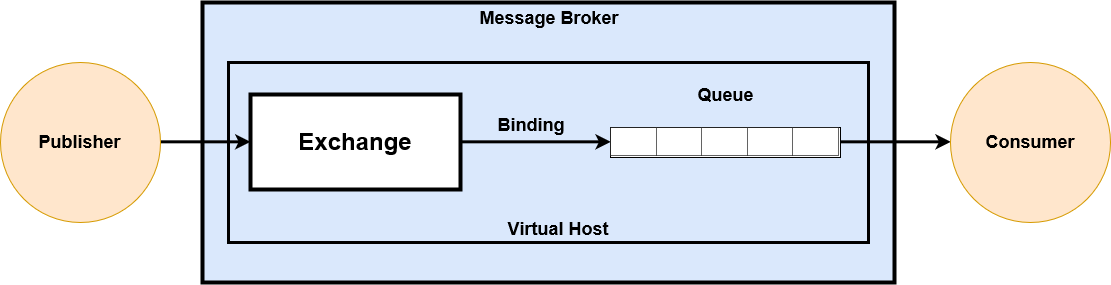
\includegraphics[width=0.4\textwidth]{AQMP_1}
\caption{AMQP model used by RabbitMQ.}
\label{fig:model}
\end{figure}

The message broker like shown in \Cref{fig:model} shows the conceptual model, including the parts of the message broker. Exchanges are endpoints where a publisher connects and sends messages to. The exchange is then responsible for the correct routing of the messages to the queues. This is done by a so called binding. It acts as a logical link between an exchange and a queue. This can be seen as a filter mechanism for messages. The queue itself stores messages and forwards them to connected consumers. Virtual hosts are an optional feature which allows to devide exchanges, bindings and queues into logical units for administration \cite{Toshev2015}.

\subsection{Exchange Types}
The most important aspect of a message broker is the routing of messages to the right consumers. This can be just a single receiver, a selection of receivers, or all possible consumers that belong to a messaging service. RabbitMQ provides four different exchange types which define the behaviour of how a message is routed by the broker.

\subsubsection{Direct Exchange}
The direct exchange uses routing keys to determine to which queue a message has to be delivered. It can only deliver a message to a queue when the routing key, which is provided in the message header, matches the binding key of a queue.
\begin{figure}[ht]
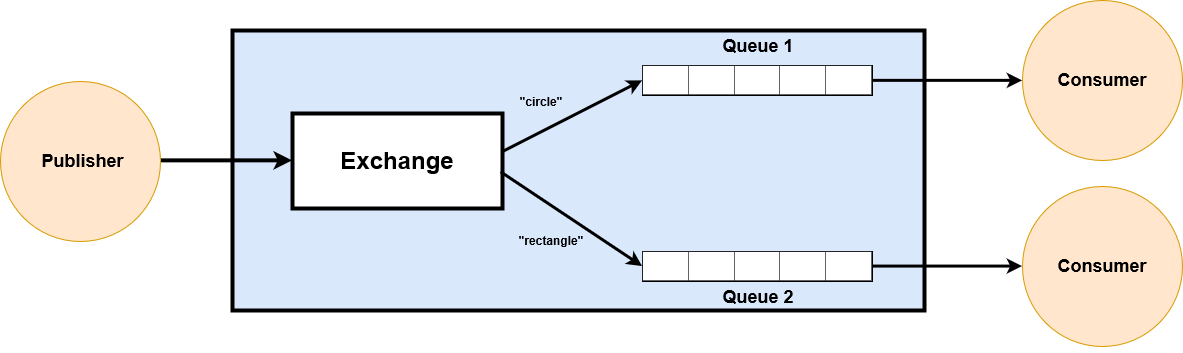
\includegraphics[width=0.4\textwidth]{direct_exchange}
\caption{RabbitMQ Direct Exchange example.}
\label{fig:direct}
\end{figure}
\Cref{fig:direct} shows a simple example where two queues are binded to a exchange, using different binding keys ("circle" and "rectangle"). If a publsiher sends a message with the routing key "rectangle" to the exchange it will then only deliver the message to Queue 2 which matches the routing key.

\subsubsection{Topic Exchange}
The topic exchange offers more freedom in specifing binding keys than the direct exchange. It provides wildcards to define patterns that can contain an asterix ("*") which is a substitute to for exactly one word, or a hash ("\#") that substitutes zero or more words. How topic exchange works can be demonstrated in a simple example:
\begin{enumerate}
	\item B1 = "car.*"
	\item B2 = "car.\#"
	\item B3 = "car"
	\item R = "car.Audi"
\end{enumerate}
The binding key B3 just matches the term "car". The binding keys of B1 and B2 are expanded using the wildcards explained above. If a publisher sends a message to the broker using the routing key R the message will just be delivered to B1 and B2, but not B3. B3 is not matching the pattern defined by the topic exchange. This can be used as a multicast mechanism.

\subsubsection{Fanout Exchange}
While the topic exchange can be used for multicast scenarios, the fanout exchange can provide a broadcast mechanism. It always delivers a message to all queues that are bounded to an exchange regardless of the underlying bindings.

\subsubsection{Headers Exchange}
The headers exchange acts like the topic exchange, but offers more flexibility. Instead of using the routing key it delivers messages to queues based on message header attributes \cite{Toshev2015}.


\subsection{Distribution of Brokers}
Developing distributed systems, the most common way is to let all machines connect to a single RabbitMQ broker. However there might be cases where one broker is not sufficient. In cases like this RabbitMQ provides mechanisms where the broker itself is distributed \cite{pivotal:distributed}. The following shows the three appreoaches which are provided.

\subsubsection{Clustering}
Clustering connects RabbitMQ brokers to a logical grouping. I can mirror whole Virtual Nodes or just exchanges across all brokers in a cluster. The user can then decide whether to locate queues on a single node, or also to mirror them. The approach of clustering provides a higher availability and increases the throughput.

\subsubsection{Federation}
Federation addresses a different need than clustering. It allows exchanges or queues on one broker to receive messages that are sent to another exchange or queue on a different broker. This allows to connect brokers through the internet and provides the delivery of messages between them.

\subsubsection{The Shovel}
The Shovel works similar to the Federation but it provides more control. It simply consumes messages and forwards them to the exchange of another broker. This is done in a lower level than the Federation does.

\subsection{Summary}
RabbitMQ and its underlying AMQP model represent a great message broker for distributed systems. Different exchange types provide filter mechanisms that allow routing rules for different needs. AMQP decouples the message delivery from the used programming language. In addition to that mechanisms for error handling and guaranteed delivery of messages make RabbitMQ a great messaging service. It's not just open source it can also easily extended by plugins. These provide for example additional messaging protocols like STOMP and MQTT, which will be briefly described in \Cref{sec:protocols}.

\section{Comparison}

\subsection{Clustering}

\subsection{Messaging Protocols}
\label{sec:protocols}

\subsection{Message Delivery Performance}

